\documentclass{standalone}
\usepackage{tikz}
\begin{document}
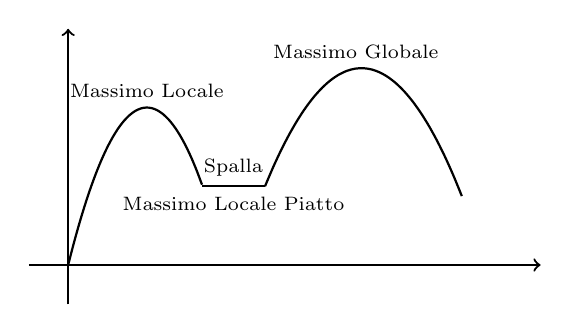
\begin{tikzpicture}[scale=2]
    \draw[->, thick](-0.25,0)--(3,0);
    \draw[->, thick](0,-0.25)--(0,1.5);
    \draw[thick]plot[smooth, domain=0:0.85](\x, {-((\x-1/2)*2)^2+1});
    \draw[thick](0.85,0.5)--(1.25,0.5)node[midway, below, align=center]{\scriptsize Massimo Locale Piatto}node[midway, above]{\scriptsize Spalla};
    \draw[thick]plot[smooth, domain=1.25:2.5](\x,{-0.5*((\x-3.725/2)*2)^2+1.25});
    \draw 
    (0.5,1)node[above]{\scriptsize Massimo Locale}
    (1.8265, 1.25)node[above]{\scriptsize Massimo Globale}
    ;
\end{tikzpicture}
\end{document}